\section{实验原理}

该部分主要阐明实验所采用的一些方法,主要针对数据的处理,最终训练模型从而实现预测功能。

\subsection{傅里叶变换}

傅立叶变换是一种分析信号的方法,它可分析信号的成分,也可用这些成分合成信号。
$f(t)$是$t$的周期函数,如果$t$满足以下条件:在一个以$2T$为周期内$f(t)$连续或只有有限个第一类间断点,
且$f(t)$单调或可划分成有限个单调区间,则$f(t)$以$2T$为周期的傅里叶级数收敛,
和函数$F(\omega)$也是以$2T$为周期的周期函数,且在这些间断点上函数是有限值;在一个周期内具有有限个极值点;绝对可积。
下列公式即称为积分运算$f(t)$的傅立叶变换:

\begin{figure}[ht]
	\centering
	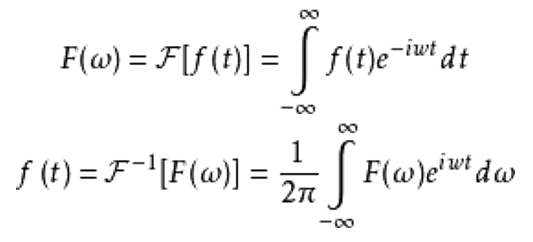
\includegraphics[width=.6\linewidth]{fft}
	\caption{连续函数傅里叶变换}
	\label{fig:fft}
\end{figure}

$f(t)$式的积分运算叫做$F(\omega)$的傅立叶逆变换。$F(\omega)$叫做$f(t)$的像函数,
$f(t)$叫做$F(\omega)$的像原函数。$F(\omega)$是$f(t)$的像。$f(t)$是$F(\omega)$原像。

由于采样值为离散数据,故而该实验采用的是离散傅里叶变换。离散傅里叶变换(DFT),
是傅里叶变换在时域和频域上都呈现离散的形式,将时域信号的采样变换为在离散时间傅里叶变换(DTFT)频域的采样。
在实际应用中通常采用快速傅里叶变换以高效计算DFT。

\begin{figure}[ht]
	\centering
	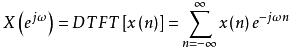
\includegraphics[width=.6\linewidth]{dtft}
	\caption{离散时间傅里叶变换}
	\label{fig:dtft}
\end{figure}

简言之,傅里叶变化就是将基于时域的特征转换成基于频域的特征。
而离散傅里叶变换就是在其基础上对离散数据基于时间进行傅里叶变换。

\subsection{主成分分析PCA}

从下图不难看出,主成分分析是将原来的变量重新组合成一组新的互相无关的变量,
同时根据实际需要从中可以取出几个较少的变量尽可能多地反映原来变量的信息的统计方法。

\begin{figure}[ht]
	\centering
	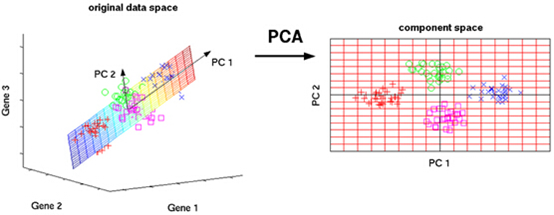
\includegraphics[width=.9\linewidth]{pca}
	\caption{主成分分析原理}
	\label{fig:pca}
\end{figure}

主成分分析能降低所研究的数据空间的维数。即用研究$m$维的$Y$空间代替$p$维的$X$空间$(m<p)$,
而低维的$Y$空间代替高维的$X$空间所损失的信息很少。

\subsection{人工神经网络的基本思想}

根据对自然神经系统构造和机理的认识,神经系统是由大量的神经细胞构成的复杂的网络,
人们对这一网络建立一定的数学模型和算法,设法使它能够实现诸如基于数据的模式识别、
函数映射等带有“智能”的功能。

\subsubsection{全连接神经网络}

对$n-1$层和$n$层而言,$n-1$层的任意一个节点,都和第$n$层所有节点有连接。
即第n层的每个节点在进行计算的时候,激活函数的输入是$n-1$层所有节点的加权。

全连接是较好的神经网络模式,但是网络很大的时候,训练速度会很慢。
部分连接就是人为切断某两个节点直接的连接,这样训练时计算量将大为减小。

\subsubsection{BP神经网络}

单个感知器能够解决线性可分的问题,但是也只能解决所谓一阶谓词逻辑问题。
所以提出了多层模型:前一层神经元的输出是后一层神经元的输入,最后一层只有一个神经元,
它接收来自前一层的$n$个输入,给出作为决策的一个输出。